\chapter{函数的极限}


在学习数列极限的基础上,本章进一步学习以实数$x$为自变量的函数$f(x)$的极限.

\section{函数的极限}
在研究无穷数到$\{a_n\}$的极限时,如果数列有通项公式,那么这个通项表达式就是一个关于自然数$n$的函数式,例如
$a_n=\frac{n+1}{n}$. 求数列$\{a_n\}$的极限,也
就是求这个函数的极限. 即
\[\lim_{n\to\infty}a_n = \lim_{n\to\infty}\frac{n+1}{n}=\lim_{n\to\infty}\left(1+\frac{1}{n}\right)=1\]

而对于函数$f(x)=\frac{x+1}{x}\; (x\ne 0)$,当自变量$x\to \infty$时函数的变化趋势是什么含义呢?

由于$f(x)=\frac{x+1}{x}=1+\frac{1}{x}$,观察函数$y=f(x)=\frac{x+1}{x}$的图象(如图11.1)可以看出:
\begin{figure}[htp]
    \centering
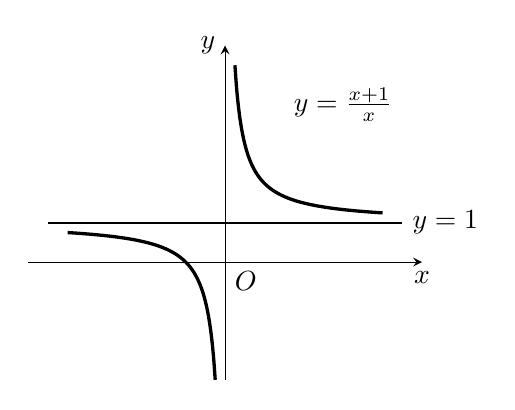
\begin{tikzpicture}[>=stealth, scale=.5]
\draw[->](-5,0)--(5,0)node[below]{$x$};
\draw[->](0,-3)--(0,5.5)node[left]{$y$};
\draw[thick](-4.5,1)--(4.5,1)node[right]{$y=1$};
\node [below right]{$O$};
\draw[domain=.25:4, smooth, samples=100, very thick]plot(\x, {1+1/\x});
\draw[domain=-4:-.25, smooth, samples=100, very thick]plot(\x, {1+1/\x});
\node at (3,4){$y=\frac{x+1}{x}$};
\end{tikzpicture}
    \caption{}
\end{figure}



若 $x>0$, 则$\frac{x+1}x>1$, 且当 $x$ 的值无限增大(记作 $x\to+\infty$)时,有$\frac{1}{x}$的值无限趋近于$0\; \left(\text{记作}\frac{1}{x}\to 0\right)$, 所以$1+\frac{1}{x}$的值
无限趋近于$1\; \left(\text{记作 }1+\frac1x\to1\right)$. 我们称,当 $x\to+\infty$时,$\frac{x+1}x$ 的极限值为 1, 记作$\lim\limits_{x\to+\infty}\frac{x+1}{x}=1$.

若 $x< 0$, 则$\frac{x+1}x<1$,且当 $x$ 的绝对值无限增大(记作 $x\to -\infty$)时 , 有 $\frac 1x\to 0$, 所 以$1+ \frac 1x\to 1$, 我 们 称 当 $x\to -\infty$ 时, $\frac{x+1}{x}$的极限值为 1, 记作$\lim\limits_{x\to-\infty}\frac{x+1}{x}=1$.

若$x$的值可以为正、也可以为负,且当$x$的绝对值无限增大(记作 $x\to \infty$ )时 , 有$\frac 1x\to 0$, 所 以$1+ \frac 1x\to 1$. 我们称$x\to\infty$ 时,$\frac{x+1}x$的极限值为 1. 记作$\lim\limits_{x\to\infty}\frac{x+1}x=1$.

一般地,对于函数 $y=f(x)$, 当自变量 $x$ 的绝对值无限增大时,若 $f(x)$的值无限趋近于一个常数 $A$, 则称 $x\to\infty$时,函数 $f(x)$的极限是 $A$, 记作$\lim\limits_{x\to\infty} f(x)=A$.

另外,当$x\to+\infty$时,若$f(x)\to A$($A$为常数),记作$\lim\limits_{x\to+\infty}f(x)=A$; 当 $x\to-\infty$时,若 $f(x)\to A$($A$ 为常数),记作$\lim\limits_{x\to-\infty}f(x)=A$.

根据函数极限的定义,若$f(x)=C$($C$为常数),显然$\Lim{x}{\infty}f(x)=C$.

\begin{example}
根据函数极限的定义及函数的图象,说出下列极限.
\begin{multicols}{2}
\begin{enumerate}[(1)]
    \item $\Lim{x}{-\infty}(2^x+1)$
    \item $\Lim{x}{-\infty}(2^{-x}-1)$
    \item $\LIM{x}\frac{-x}{x+2}$
    \item $\Lim{x}{+\infty}(2^x+1)$
\end{enumerate}    
\end{multicols}
\end{example}

\begin{solution}
\begin{enumerate}[(1)]
\begin{minipage}{.45\textwidth}
\item 作函数$y=2^x+1$的图象(如图11.2).

    $\because\quad$当$x\to - \infty$时, $2^{x}\to 0$,

$\therefore\quad 2^{x}+1\to1$

$\therefore\quad \lim\limits_{n\to -\infty }( 2^{x}+ 1) = 1$
\end{minipage}
\hfill
\begin{minipage}{.45\textwidth}
\centering
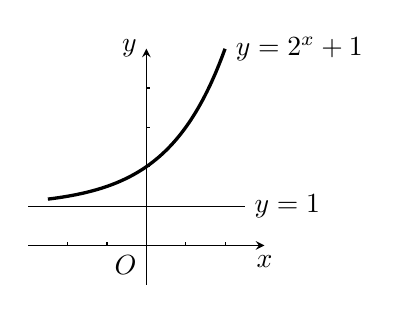
\begin{tikzpicture}[>=stealth, scale=.5]
\draw[->](-3,0)--(3,0)node[below]{$x$};
\draw[->](0,-1)--(0,5)node[left]{$y$};
\node[below left]{$O$};
\draw(-3,1)--(2.5,1)node[right]{$y=1$};
\draw[domain=-2.5:2, samples=100, smooth, very thick]plot(\x, {2^(\x)+1})node[right]{$y=2^{x}+1$};
\foreach \x in {-1,-2,1,2}
{
    \draw(\x,0)--(\x,.1);
}
\foreach \x in {1,2,3,4}
{
    \draw(0,\x)--(.1,\x);
}
\end{tikzpicture}
\captionof{figure}{}
\end{minipage}

\begin{minipage}{.45\textwidth}
\item 作函数$y=2^{-x}-1$的图象(如图11.3).

$\because\quad $当$x\to + \infty$ 时, $2^{- x}\to 0$,

$\therefore\quad 2^{-x}-1\to-1$

$\therefore\quad \lim\limits_{x\to + \infty }( 2^{- x}- 1) = - 1$
\end{minipage}
\hfill
\begin{minipage}{.45\textwidth}
\centering
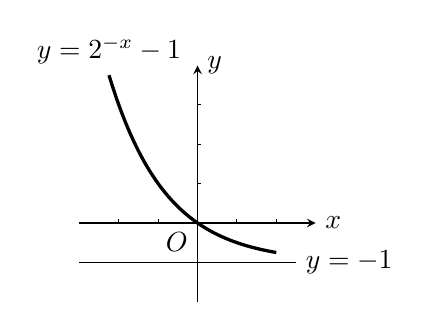
\begin{tikzpicture}[>=stealth, scale=.5]
\draw[->](-3,0)--(3,0)node[right]{$x$};
\draw[->](0,-2)--(0,4)node[right]{$y$};
\node[below left]{$O$};
\draw(-3,-1)--(2.5,-1)node[right]{$y=-1$};
\draw[domain=2:-2.25, samples=100, smooth, very thick]plot(\x, {2^(-\x)-1})node[above]{$y=2^{-x}-1$};
\foreach \x in {-1,-2,1,2}
{
    \draw(\x,0)--(\x,.1);
}
\foreach \x in {1,2,3}
{
    \draw(0,\x)--(.1,\x);
}
\end{tikzpicture}
\captionof{figure}{}
\end{minipage}
    
\item 作函数$y=\frac{-x}{x+2}$的图象(如图11.4).

$\because\quad f(x)=\frac{-x}{x+2}=-1+\frac{2}{x+2}$,
当 $x\to \infty$ 时 , $\frac 2{x+ 2}\to 0$

$\therefore\quad - 1+ \frac 2{x+ 2}\rightarrow - 1$

$\therefore\quad \lim\limits_{x\to \infty }\frac {- x}{x+ 2}= - 1$

\begin{figure}[htp]
    \centering
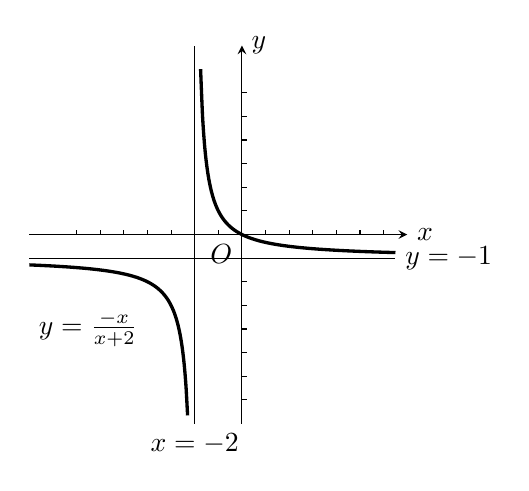
\begin{tikzpicture}[>=stealth, scale=.3]
\draw[->](-9,0)--(7,0)node[right]{$x$};
\draw[->](0,-8)--(0,8)node[right]{$y$};
\node[below left]{$O$};
\draw(-9,-1)--(6.5,-1)node[right]{$y=-1$};
\draw(-2,-8)node[below]{$x=-2$}--(-2,8);
\draw[domain=-1.75:6.5, samples=100, smooth, very thick]plot(\x, {-\x/(\x+2)});
\draw[domain=-9:-2.3, samples=100, smooth, very thick]plot(\x, {2/(\x+2)-1});

\foreach \x in {-7,-6,...,6}
{
    \draw(\x,0)--(\x,.2);
    \draw(0,\x)--(.2,\x);
}
\node at (-4,-4)[left]{$y=\frac{-x}{x+2}$};

\end{tikzpicture}
    \caption{}
\end{figure}


\item $\because\quad $当 $x\to + \infty$ 时 , $2^{x}+ 1$ 的值无限增大,即 $2^x+1\to+\infty$(如图11.2).

$\because\quad $当 $x\to+\infty$时, $f(x)=2^x+1$ 的值不是无限趋近一个常数,

$\therefore\quad \lim\limits_{x\to + \infty }\left ( 2^x+ 1\right )$不存在. 
\end{enumerate}
\end{solution}


一般地,对于函数 $y=f(x)$, 当 $x\to\infty$时,若$|f(x)|\to+\infty$或 $f(x)$的值不是无限趋近一个
常数 $A$, 那么称当 $x\to\infty$时, $f( x)$ 的 极 限 不 存 在.

在本节开始,对于函数$y=\frac{x+1}{x}\; (x\neq0)$, 我们已经解决了
当 $x\to\infty$时,$f(x)$的变化趋势. 而当 $x\to x_0$ ($x_{0}$ 为给定的常数)
时,$f(x)$的变化趋势如何?

对于函数 $f(x)=2x+1$, 当 $x\to3$ 时,有 $2x+1\to7$, 我们
称 $f(x)$的极限值为 7, 即$\lim\limits_{x\to3}f(x)=7$.

下面再研究函数$y=\frac{x^{2}-1}{x-1}$ 在点 $x=1$ 处的变化趋势.

$\because\quad$ 当$x\neq1$时, $y=\frac{x^{2}-1}{x-1}=x+1$.

$\therefore\quad$ 观察函数 $y=\frac{x^{2}-1}{x-1}$ 的图象(如图 11.5)可知, 此函数图象是一条在点 $A(1,2)$处有个“洞”的直线.

\begin{figure}[htp]
    \centering
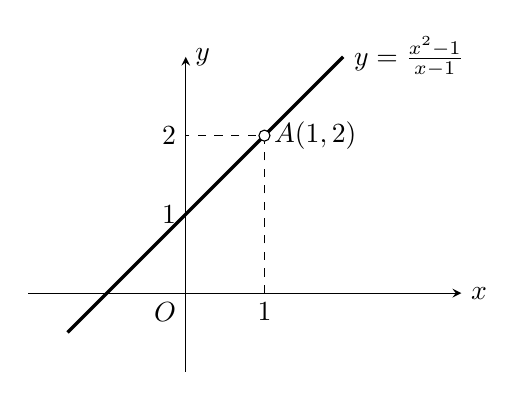
\begin{tikzpicture}[>=stealth]
\draw[->](-2,0)--(3.5,0)node[right]{$x$};    
\draw[->](0,-1)--(0,3)node[right]{$y$}; 
\draw[domain=-1.5:2, smooth, very thick]plot(\x, {\x+1})node[right]{$y=\frac{x^{2}-1}{x-1}$};
\draw[dashed](1,0)node[below]{1}--(1,2)node[right]{$A(1,2)$}--(0,2)node[left]{2};
\draw[fill=white](1,2)circle(2pt);
\node[below left]{$O$};
\node at (0,1)[left]{1};
\end{tikzpicture}
    \caption{}
\end{figure}

若$x> 1$, 则$\frac {x^{2}- 1}{x- 1}> 2$, 且当 $x$的值 无 限 趋 近 于 1(记作 $x\to 1^{+ }$)时 , 有 $x+ 1\to 2$, 所 以 $\frac {x^{2}- 1}{x- 1}\to 2$. 我 们 称 当  $x\to 1^{+ }$时 , $\frac {x^{2}- 1}{x- 1}$的 极 限 值 为  2, 记 作
$\lim\limits_{x\to1^+}\frac{x^2-1}{x-1}=2$.

若 $x<1$, 则$\frac{x^{2}-1}{x-1}<2$, 且当 $x$ 的值无限趋近于 1(记作
$x\to 1^{- }$) 时 , 有$x+ 1\to 2$, 所 以$\frac {x^{2}- 1}{x- 1}\to 2$. 我们称当$x\to1^-$时, 
$\frac{x^2-1}{x-1}$的极限值为 2, 记作$\lim\limits_{x\to1^-}\frac{x^2-1}{x-1}=2$.

当$x\neq1$且$x$的值无限趋近于 1(这时$x$的值大于1 或小于1,记作 $x\to1$)时,因为 $x+1\to2$, 所以$\frac{x^{2}-1}{x-1}\to2$. 我们称当
$x\to1$ 时, $\frac{x^{2}-1}{x-1}$的极限值为 2, 记作$\lim\limits_{x\to1}\frac{x^{2}-1}{x-1}=2$.

一般地,已知函数 $y=f(x)$在点 $x=x_0$ 的附近有定义,当自变量$x$取不同于$x_0$的值且无限地趋近于$x_0$时,若$f(x)$的值无限地趋近于一个常数 $A$, 则称当 $x\to x_0$ 时,函数 $f(x)$的极限值是 $A$, 记作 $\lim_{x\to x_0}\limits f(x)=A$.

另外,当$x\to x_0^-$时,若$f(x)\to A$($A$为常数), 我们称函数$f(x)$在点 $x=x_0$ 处有左极限,记作$\lim\limits_{x\to x_{0}^-}f(x)=A$; 当$x\to x_{0}^{+}$ 时,若$f(x)\to A$($A$为常数), 我们称函数$f(x)$在点$x=x_0$处有右极限,记作$\lim\limits_{x\to x^+_0}f(x)=A$.

\begin{example}
根据函数的极限定义及函数的图象,说出下列函
数指定的极限。
\begin{multicols}{2}
\begin{enumerate}[(1)]
    \item $ \lim\limits _{x\to 1^{- }}\left ( x^{2}- 1\right )$
    \item $\lim\limits _{x\to - 1^{+ }}\left ( x^{2}- 1\right )$
    \item $\lim\limits _{x\to 0}( x^{2}- 1)$
    \item $\lim\limits _{x\to \tfrac 12}( x^{2}- 1) $
\end{enumerate}
\end{multicols}
\end{example}

\begin{solution}
设$f( x) = x^2- 1\; (x\in [ - 1,1])$. 作函数 $y= x^2- 1\; ( x\in [ - 1, 1] )$的 图 象 (如 图  11.6) , 观 察 图 象 可 知 : 

\noindent
\begin{minipage}{.5\textwidth}
\begin{enumerate}[(1)]
    \item $\because\quad $当$x\to1^-$时,$x^2-1\to0$.
    
    $\therefore\quad \lim\limits_{x\to 1^{- }}( x^{2}- 1) = 0.$
    
\item      $\because\quad $当$x\to -1^+$时,$x^2-1\to0$.
    
   $\therefore\quad \lim\limits_{x\to 1^{+ }}( x^{2}- 1) = 0$

   \item      $\because\quad $当$x\to 0$时,$x^2-1\to-1$.
    
   $\therefore\quad \lim\limits_{x\to 0}( x^{2}- 1) = -1$

   \item      $\because\quad $当$x\to \frac{1}{2}$时,$x^2-1\to -\frac{3}{4}$.
    
   $\therefore\quad \lim\limits_{x\to \tfrac{1}{2}}( x^{2}- 1) = -\frac{3}{4}$
\end{enumerate}    
\end{minipage}
\hfill
\begin{minipage}{.4\textwidth}
    \centering
\begin{tikzpicture}[>=stealth]
\draw[->](-2,0)--(2,0)node[below]{$x$};
\draw[->](0,-2)--(0,1.5)node[left]{$y$};
\draw[domain=-1:1, smooth, very thick]plot(\x, {\x*\x-1});
\foreach \x in {-1,1}
{
    \draw[fill](\x,0)node[above]{$\x$} circle(1pt);
}
\draw(.5,-.75)--(.5,0)node[above]{$\frac{1}{2}$};
\node at (0,-1)[below left]{$-1$};
\node[below left]{$O$};
\end{tikzpicture}
\captionof{figure}{}
\end{minipage}

\end{solution}

\begin{example}
已知:函数$f(x)=\begin{cases}
    2-x,& x\ge 1\\
    -1,& -1<x<1\\
    1+x,& x\le -1
\end{cases}$

根据函数的极限定义及函数的图象,说出下列函数指定
的极限。
\begin{multicols}{3}
\begin{enumerate}[(1)]
    \item $\Lim{x}{1^+}f(x)$
    \item $\Lim{x}{1^-}f(x)$
    \item $\Lim{x}{-1^+}f(x)$
    \item $\Lim{x}{-1^-}f(x)$
    \item $\Lim{x}{-2}f(x)$
    \item $\Lim{x}{2}f(x)$
\end{enumerate}
\end{multicols}
\end{example}

\begin{solution}
作函数$y=f(x)$的图象(如图11.7)

\begin{multicols}{2}
    \begin{enumerate}[(1)]
\item $\because\quad$ 当  $x\to 1^{+ }$时, $2-x\to1$

$\therefore\quad \lim\limits _{x\to 1^{+ }}f( x) = 1$

\item $\because\quad$ 当$x\to1^-$时, $f(x)=-1$,

$\therefore\quad\lim\limits _{x\to 1^{-}} f(x)=-1.$

\item $\because\quad$ 当$x\to-1^+$时, $f(x)=-1$

$\therefore\quad\lim\limits_{x\to - 1^{+ }}f( x) = - 1.$ 

\item $\because\quad$ 当  $x\to -1^{- }$时, $1+x\to 0$

$\therefore\quad \lim\limits _{x\to -1^{- }}f( x) = 0$

\item $\because\quad$ 当$x\to -2$时, $1+x\to -1$,

$\therefore\quad\lim\limits _{x\to -2} f(x)=-1.$

\item $\because\quad$ 当$x\to 2$时, $2-x\to 0$

$\therefore\quad\lim\limits_{x\to 2}f( x) = 0.$ 
\end{enumerate}
\end{multicols}

\end{solution}

\begin{figure}[htp]
    \centering
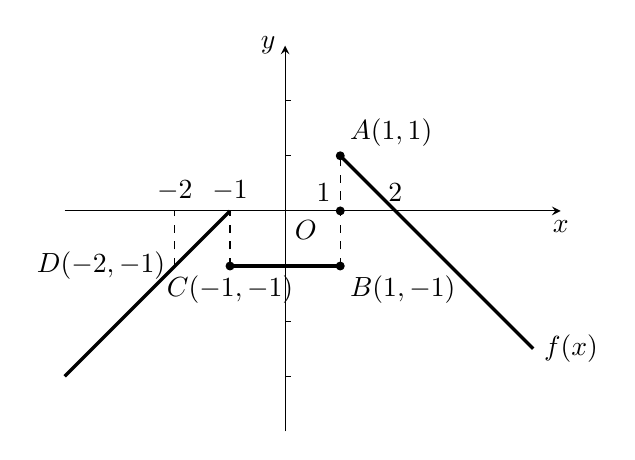
\begin{tikzpicture}[>=stealth, scale=.7]
\draw[->](-4,0)--(5,0)node[below]{$x$};
\draw[->](0,-4)--(0,3)node[left]{$y$};
\draw[domain=-4:-1, smooth, very thick]plot(\x, {\x+1});
\draw[domain=1:4.5, smooth, very thick]plot(\x, {-\x+2})node[right]{$f(x)$};
\draw[domain=-1:1, smooth, very thick]plot(\x, -1);

\foreach \x/\y in {1/0, -1/-1, 1/-1, 1/1}
{
    \draw[fill](\x,\y) circle(2pt);
}
\node at (-2,-1)[left]{$D(-2,-1)$};
\node at (-1,-1)[below]{$C(-1,-1)$};
\node at (1,-1)[below right]{$B(1,-1)$};
\node at (1,1)[above right]{$A(1,1)$};

\foreach \x in {2,-1,-2}
{
    \node at (\x,0)[above]{$\x$};
}
\node at (1,0)[above left]{1};
\draw[dashed](-2,-1)--(-2,0);
\draw[dashed](1,-1)--(1,1);
\draw[dashed](-1,-1)--(-1,0);

\foreach \x in {-3,-2,-1,1,2}
{
    \draw(0,\x)--(.1,\x);
}

\node[below right]{$O$};
\end{tikzpicture}    
    \caption{}
\end{figure}

根据函数的极限的定义,不难得出:
\begin{enumerate}
    \item 若函数 $f(x)$在点 $x=x_0$ 处附近有定义则$\lim\limits_{x\to x_{0}}f(x)=A$的 充 分 必 要 条 件 是$\lim\limits _{x\to x^-_0 }f( x) = A$且$\lim\limits_{x\to x^+_0}f(x)=A$(其中$A$为常数).
    \item 对于函数$f(x)=C$($C$为常数)及任一给定的常数$x_0$, 恒有$\lim\limits_{x\to x_0}f(x)=c$.
    
现在我们看函数$f(x)=\frac{x+1}{x}$在点$x=0$处附近的变化趋势. 由函数$y=\frac{x+1}{x}$的图象(如图 11.1)可知:
\begin{itemize}
\item 当$x\to0^{+}$时, $\frac{x+1}x>0$且$\frac{x+1}x$的值无限增大,所以
$\lim\limits_{x\to0^+}\frac{x+1}x$不存在.
\item 
当$x\to0^{-1}$时, $\frac{x+1}x<0$且$\left|\frac{x+1}x\right|$的值无限增大,所以
$\lim\limits_{x\to0^-}\frac{x+1}x$也不存在.
\end{itemize}
我们也可以说当 $x\to0$ 时,$\lim\limits_{x\to0}\frac{x+1}x$不存在.
\end{enumerate}

\subsection*{练习}
\begin{enumerate}
    \item 根据函数的极限定义和函数的图象,写出下列各极限。
\begin{multicols}{2}
\begin{enumerate}[(1)]
    \item $\lim\limits_{x\to+\infty}(1-2^{-x})$
    \item $\lim\limits_{x\to+\infty}|2^{-x}-1|$
\item $\lim\limits_{x\to\infty}\frac{2x}{x-1}$
\item $\lim\limits _{x\to 0}|x|$
\item $\lim\limits _{x\to - 1}( - x+ 1)$
\item $\lim\limits_{x\to-1}\frac{x^2-1}{x+1}$
\item $\lim\limits _{x\to  1}( - x+ 1)$
\item $\lim\limits _{x\to  1}\frac{x^2-1}{x+1}$
\end{enumerate}
\end{multicols}

\begin{tikzpicture}[>=stealth, scale=.4]
\begin{scope}
    \draw[->](-4,0)--(5,0)node[below]{$x$};
    \draw[->](0,-4)node[below]{第(1)题}--(0,3)node[left]{$y$};
\draw (-4,1)--(5,1)node[above]{$y=1$};
\draw[domain=3:-2, smooth, very thick]plot(\x, {1-2^(-\x)})node[below left]{$y=1-2^{-x}$};
\node [below right]{$O$};
\foreach \x  in {1,2,3}
{
    \draw(\x,0)--(\x,.1);
    \draw(0,-\x)--(.1,-\x);
}
\end{scope}
\begin{scope}[xshift=13cm, yshift=-2cm]
    \draw[->](-4,0)--(5,0)node[below]{$x$};
\draw[->](0,-2)node[below]{第(2)题}--(0,5)node[left]{$y$};
\draw(-4,1)--(5,1)node[above]{$y=1$};
\draw[domain=0:3, smooth, very thick]plot(\x, {1-2^(-\x)});
\draw[domain=0:-2.2, smooth, very thick]plot(\x, {2^(-\x)-1});
\node at (-3,3)[above]{$y=|2^{-x}-1|$};
\node [below left]{$O$};
\foreach \x  in {-1,1,2,3,4}
{
    \draw(\x,0)--(\x,.1);
    \draw(0,\x)--(.1,\x);
}

\end{scope}
\end{tikzpicture}

\begin{tikzpicture}[>=stealth]
\begin{scope}[scale=.45]
    \draw[->](-4,0)--(5,0)node[below]{$x$};
    \draw[->](0,-4)node[below]{第(3)题}--(0,5)node[left]{$y$};
\draw (-4,2)--(5,2)node[below]{$y=2$};
\draw (1,-3.5)node[right]{$x=1$}--(1,5);
\draw[domain=1.7:5, smooth, very thick]plot(\x, {2+2/(\x-1)});
\draw[domain=.6:-4, smooth, very thick]plot(\x, {2+2/(\x-1)});
\node [below left]{$O$};
\foreach \x  in {-3,-1,-2,1,2,3}
{
    \draw(\x,0)--(\x,.1);
    \draw(0,\x)--(.1,\x);
}
\end{scope}
\begin{scope}[xshift=6cm, yshift=-1cm]
    \draw[->](-2.5,0)--(3,0)node[below]{$x$};
\draw[->](0,-1)node[below]{第(4)题}--(0,3)node[left]{$y$};
\draw[domain=0:2, smooth, very thick]plot(\x, \x);
\draw[domain=0:-2, smooth, very thick]plot(\x, -\x);
\node at (2,2)[right]{$y=|x|$};
\node [below left]{$O$};
\foreach \x  in {1,2}
{
    \draw(\x,0)--(\x,.1);
    \draw(-\x,0)--(-\x,.1);
    \draw(0,\x)--(.1,\x);
}
\end{scope}

\end{tikzpicture}

\begin{tikzpicture}[>=stealth, scale=.6]
\begin{scope}
    \draw[->](-4,0)--(4,0)node[below]{$x$};
    \draw[->](0,-1)node[below]{第(5)(7)题}--(0,5)node[left]{$y$};
\draw[domain=1.5:-2.5, smooth, very thick]plot(\x, {-\x+1})node[above]{$y=-x+1$};
\foreach \x  in {1,2,3}
{
    \draw(\x,0)--(\x,.1);
    \draw(-\x,0)--(-\x,.1);
    \draw(0,\x)--(.1,\x);
}
\foreach \x in {-1,1}
{
    \node at (\x,0)[below]{$\x$};
}
\node at (.2,1)[right]{1};
\node [below right]{$O$};

\draw[dashed](-1,0)--(-1,2);
\end{scope}
\begin{scope}[xshift=8cm, yshift=2cm]
    \draw[->](-2.5,0)--(4,0)node[below]{$x$};
\draw[->](0,-3)node[below]{第(6)(8)题}--(0,3)node[left]{$y$};
\draw[domain=-2:3, smooth, very thick]plot(\x, \x-1)node [right]{$y=\frac{x^2-1}{x+1}$};
\draw[fill=white](-1,-2)node[right]{$A(-1,-2)$} circle(2pt);
\draw[dashed](-1,0)node[above]{$-1$}--(-1,-2);
\node [below left]{$O$};
\foreach \x  in {1,2}
{
    \draw(\x,0)--(\x,.1);
    \draw(-\x,0)--(-\x,.1);
    \draw(0,\x)--(.1,\x);
}
\node at (1,0)[below]{1};
\node at (0,-1)[right]{$-1$};
\end{scope}

\end{tikzpicture}

\noindent
\begin{minipage}{.45\textwidth}
\item 已知:$f(x)=\arccos x$, 根据函数的极限的定义和函数的图象, 写 出 下 列 各 函 数 指 定 的 极 限 . 
\begin{multicols}{2}
\begin{enumerate}[(1)]
    \item $\lim\limits _{x\to 1^- }f( x)$
    \item $\lim\limits _{x\to -1^+ }f( x)$
    \item $\lim\limits _{x\to 0^+ }f( x)$
    \item $\lim\limits _{x\to 0^- }f( x)$
    \item $\lim\limits _{x\to 0 }f( x)$
    \item $\lim\limits _{x\to \tfrac{1}{2}^+ }f( x)$
    \item $\lim\limits _{x\to \tfrac{1}{2}^- }f( x)$
    \item $\lim\limits _{x\to \tfrac{1}{2} }f( x)$
\end{enumerate}
\end{multicols}
\end{minipage}\hfill
\begin{minipage}{.45\textwidth}
\centering
\begin{tikzpicture}[>=stealth]
    \draw[->](-2.5,0)--(2.5,0)node[below]{$x$};
    \draw[->](0,-1)node[below]{第3题}--(0,4)node[left]{$y$};
\draw[dashed](-1,0)node[below]{$-1$}--(-1,pi)node[above left]{$A(-1,\pi)$}--(0,pi)node[right]{$\pi$};
\draw[dashed](.5,0)node[below]{$\frac{1}{2}$}--(.5,pi/3)node[right]{$B\left(\frac{1}{2},\frac{\pi}{3}\right)$}--(0,pi/3)node[left]{$\frac{\pi}{3}$};
\node[below left]{$O$};
\draw[domain=0:pi, smooth, samples=100, very thick]plot({cos(\x r)}, \x);
\node at (0,pi/2)[above right]{$\frac{\pi}{2}$};

\end{tikzpicture}    
\end{minipage}

\item 已知:$f(x)=\begin{cases}
    x &x\ge 0\\
-x+1 & x<0
\end{cases}$,
根据函数的极限的定义和函数的图象, 写 出 下 列 各 函 数 指 定 的 极 限 . 
\begin{multicols}{2}
\begin{enumerate}[(1)]
    \item $\lim\limits _{x\to 0^+ }f( x)$
    \item $\lim\limits _{x\to 0^- }f( x)$
    \item $\lim\limits _{x\to 2 }f( x)$
    \item $\lim\limits _{x\to -2 }f( x)$
\end{enumerate}
\end{multicols}
\end{enumerate}

\section{函数极限的四则运算法则}
函数极限与数列极限有着类似的四则运算法则,利用它们可求一些较复杂的函数的极限.

如果$\lim\limits_{x\to x_{0}}f(x)=A$, $\lim\limits_{x\to x_{0}}g(x)=B$, 那么
\begin{enumerate}
    \item $\lim\limits_{x\to x_{0}}[f(x)\pm g(x)]=\lim\limits_{x\to x_{0}}f(x)\pm\lim_{x\to x_{0}}g(x)=A\pm B$
    \item $\lim\limits_{x\to x_{0}}[f(x)\cdot g(x)]=\lim\limits_{x\to x_{0}}f(x)\cdot\lim_{x\to x_{0}}g(x)=A  B$
\begin{thm}
   {推论} $\lim\limits_{x\to x_{0}}Cf( x) = C\lim\limits _{x\to x_{0}}f( x) = CA\quad (C\text{为常数})$
\end{thm}
\item $\lim\limits_{x\to x_0}\frac{f(x)}{g(x)}=\frac{\lim\limits_{x\to x_0}f(x)}{\lim\limits_{x\to x_0}g(x)}=\frac{A}{B}$

(当$x\to x_0$时,$g(x)\ne 0$且$B\ne 0$)
\end{enumerate}

\begin{rmk}
\begin{enumerate}
    \item 函数极限的四则运算法则的实质仍是改变运算顺序,
    \item 上述函数极限的四则运算法则还可以推广到有限个
函数的和、差、积、商的情况。
\item 上述函数极限的四则运算法则对于自变量$x$来说,当
$x\to+\infty$, $x\to-\infty$, $x\to\infty$, 或 $x\to x_0^+$, $x\to x_0^-$ 等情况也是成立
的.
\end{enumerate}
\end{rmk}

\begin{example}
已知:$f(x)=3x^2-2x-1$,求$\lim\limits_{x\to 2}f(x)$.
\end{example}

\begin{solution}
    \textbf{解法1:}
\[\begin{split}
    \lim\limits_{x\to 2}f(x)&=\lim\limits_{x\to 2}(3x^2-2x-1)\\
&=\lim\limits_{x\to 2}(3x^2)-\lim\limits_{x\to 2}(2x)-\lim\limits_{x\to 2}1\\
&=3\left(\lim\limits_{x\to 2} x\right)^2 -2\lim\limits_{x\to 2} x-1\\
&=3\x 2^2-2\x 2-1 =7
\end{split} \]
    
\textbf{解法2:}
\[\begin{split}
    \lim\limits_{x\to 2}f(x)&=\lim\limits_{x\to 2}[(3x+1)(x-1)]\\
&=\lim\limits_{x\to 2}(3x+1)\cdot \lim\limits_{x\to 2}(x-1)\\
&=\left[\lim\limits_{x\to 2}(3x)+\lim\limits_{x\to 2}1\right]\left(\lim\limits_{x\to 2}x- \lim\limits_{x\to 2}1\right)\\
&=(6+1)(2-1)=7
\end{split} \]
\end{solution}

\begin{example}
已知:$f(x)=\frac{x^2-2x-3}{x^2-9}$,求
\begin{multicols}{2}
\begin{enumerate}[(1)]
    \item $\lim\limits_{x\to 3}f(x)$
    \item $\lim\limits_{x\to -3}f(x)$
\end{enumerate}
\end{multicols}
\end{example}

\begin{analyze}
\[f(x)=\frac{(x-3)(x+1)}{(x-3)(x+3)},\qquad x\in(-\infty,-3)\cup(-3,3)\cup(3,+\infty)\]
\begin{enumerate}[(1)]
    \item $\because\quad $当$x\to3$时,$x^2-9\to 0$
    
    $\therefore\quad $不能直接运用函数极限的运算法则求极限.

    由于当$x\to 3$时,$x\ne 3$即$x-3\ne 0$. 若先约去$f(x)$的分子、分母中的公因式$x-3$,则可求$f(x)$的极限.

\item $\because\quad $当$x\to-3$时,$x\ne -3$且$x+3\to 0$,而$f(x)=\frac{x+1}{x+3}=1-\frac{2}{x+3}$,这时$\left|\frac{2}{x+3}\right|\to +\infty$

$\therefore\quad f(x)$无极限.
\end{enumerate}
\end{analyze}

\begin{solution}
\begin{enumerate}[(1)]
    \item $\because\quad $当$x\to 3$时,$x-3\ne 0$

\[\begin{split}
    \therefore\quad \lim\limits_{x\to 3}f(x)&=\lim\limits_{x\to 3}\frac{(x-3)(x+1)}{(x-3)(x+3)}
    =\lim\limits_{x\to 3}\frac{x+1}{x+3}\\
    &=\frac{\lim\limits_{x\to 3}(x+1)}{\lim\limits_{x\to 3}(x+3)}=\frac{3+1}{3+3}=\frac{2}{3}
\end{split} \]


\item $f(x)=\frac{x+1}{x+3}=1-\frac{2}{x+3}$

又$\because\quad $当$x\to -3$时,$x+3\to 0$

$\therefore\quad \frac{2}{x+3}\to \infty$

$\therefore\quad 1-\frac{2}{x+3}\to\infty$,即$\lim\limits_{x\to-3}f(x)$不存在.
\end{enumerate}
\end{solution}

\begin{example}
    已知$f(x)=\frac{3x^{2}+2x-1}{4x^{2}-100x}$, 求$\lim\limits_{x\to\infty}f(x)$.    
\end{example}

\begin{analyze}
    因为当$x\to\infty$时, $f(x)$的分子, 分母都无极限. 所以不能直接运用函数根据的运算法则求极限.

    又$x\neq0$, 故可像求数列的极限一样, 先将$f(x)$的分子、分母同除以$x$的最高次幂后, 再求极限.
\end{analyze}

\begin{solution}
\[\begin{split}
    \lim\limits_{x\to\infty}f(x)&=\lim\limits_{x\to\infty}\frac{3x^{2}+2x-1}{4x^{2}-100x}=\lim\limits_{x\to\infty}\frac{3+\frac{2}{x}-\frac{1}{x^{2}}}{4-\frac{100}{x}}\\
    &=\frac{\lim\limits_{x\to\infty}\left(3+\frac{2}{x}-\frac{1}{x^{2}}\right)}{\lim\limits_{x\to\infty}\left(4-\frac{100}{x}\right)}=\frac{3+\lim\limits_{x\to\infty}\frac{2}{x}-\lim\limits_{x\to\infty}\frac{1}{x^2}}{4-\lim\limits_{x\to\infty}\frac{100}{x}}=\frac{3}{4}.
\end{split}\]
\end{solution}

\begin{example}
已知:$f(x)=\frac{1}{x-2}-\frac{3}{x^3-8}$,求$\Lim{x}{2}f(x)$.
\end{example}

\begin{analyze}
$\because\quad $当$x\to 2$时,$\frac{1}{x-2}\to\infty$, $\frac{3}{x^3-8}\to\infty$

$\therefore\quad $不能直接运用函数极限的四则运算法法则求$f(x)$的极限,应将$f(x)$的解析式先合并成一个分式,看它的分子、分母能否约去$x-2$的因式.
\end{analyze}

\begin{solution}
\[\begin{split}
\because\quad f(x)&=\frac{1}{x-2}-\frac{3x+6}{x^3-8}=\frac{x^2+2x+4-(3x+6)}{(x-2)(x^2+2x+4)}\\
&=\frac{x^2-x-2}{(x-2)(x^2+2x+4)}=\frac{(x-2)(x+1)}{(x-2)(x^2+2x+4)}
\end{split}\]
而当$x\to 2$时,$x-2\ne 0$
\[\begin{split}
\therefore\quad \Lim{x}{2}f(x)&=\Lim{x}{2}\frac{(x-2)(x+1)}{(x-2)(x^2+2x+4)}=\Lim{x}{2} \frac{x+1}{x^2+2x+4}\\
&=\frac{\Lim{x}{2}(x+1)}{\Lim{x}{2}(x^2+2x+4)}=\frac{\Lim{x}{2}x+1}{\Lim{x}{2}x^2+\Lim{x}{2}2x+4}\\
&=\frac{2+1}{4+4+4}=\frac{1}{4}
\end{split}\]
\end{solution}

\section*{习题一}
\begin{center}
\bfseries A
\end{center}

\begin{enumerate}
    \item 根据函数的极限的定义及函数的图象,分别写出下列各极限:
\begin{multicols}{3}
\begin{enumerate}[(1)]
    \item $\Lim{x}{\infty}x^{-2}$
    \item $\Lim{x}{+\infty}\left(\frac{1}{2}\right)^x$
    \item $\Lim{x}{+\infty}\arctan x$
    \item $\Lim{x}{-\infty}\arctan x$
    \item $\Lim{x}{\tfrac{\pi}{2}}\sin x$
    \item $\Lim{x}{0} \cos x$
\end{enumerate}
\end{multicols}

\item 已知:$f(x)=\begin{cases}
    (x-1)^2 & x>0\\
    0& x=0\\
    -(x+1)^2 & x<0
\end{cases}$,作函数$y=f(x)$的图象,写出下列各极限:
\begin{multicols}{4}
\begin{enumerate}[(1)]
    \item $\Lim{x}{1}f(x)$
    \item $\Lim{x}{-1}f(x)$
    \item $\Lim{x}{0}f(x)$
    \item $\Lim{x}{2}f(x)$
\end{enumerate}
\end{multicols}

\item 利用函数极限的四则运算法则求下列极限:
\begin{multicols}{2}
\begin{enumerate}[(1)]
    \item $\LIM{x}\frac{3x+1}{x^2-4}$
    \item $\LIM{x}\frac{x^2+x-1}{2x^2+5}$
    \item $\LIM{x}\frac{3x^2-2x+4}{2x+1}$
    \item $\Lim{x}{1}(5x^2-2x+7)$
    \item $\Lim{x}{-1}\frac{x^3+1}{x+1}$
    \item $\Lim{x}{2}\frac{x^2-x-2}{x^2-2x}$
    \item $\Lim{x}{1}\frac{x^2+x-2}{x^2-3x+2}$
    \item $\Lim{x}{1}\left(\frac{2}{x-1}-\frac{x+3}{x^2-1}\right)$
    \item $\Lim{x}{0}\frac{x^2+x}{2x^2-x}$
    \item $\Lim{x}{0}\left(1-\frac{2x^2-3x}{x}\right)$
\end{enumerate}
\end{multicols}
\end{enumerate}

\section{函数的连续性}
在11.2节中求函数$f(x)=3x^2-2x-1$在点$x=2$处的极限值时,我们发现
\[\lim_{x\to 2}f(x)=\lim_{x\to 2}(3x^2-2x-1)=3\x2^2-2\x2-1=7\]
而$f(2)$的值也是7.

这是不是偶然的巧合?当任取$x_0\in\R$,求函数$f(x)=3x^2-2x-1$在点$x=x_0$处的极限值时,通过计算仍有$Lim{x}{x_0}f(x)=3x^2_0-2x_0-1=f(x_0)$. 具有这种性质的函数就是本节要研究的连续函数.

下面先给出函数在某一点处连续的定义.

已知函数$y=f(x)$及点$x=x_0$,如果函数$f(x)$满足以下3个条件:
\begin{enumerate}
\item $f(x)$在点$x=x_0$处及其附近有定义;
\item $\Lim{x}{x_0}f(x)$存在;
\item $\Lim{x}{x_0}f(x)=f(x_0)$.
\end{enumerate}

那么称函数$f(x)$在点$x=x_0$处连续.

根据这个定义,如果一个函数$y=f(x)$在点$x=x_0$处不能完全满足上述3个条件,那么此函数在这个点就不连续,这时称点$x=x_0$是函数$f(x)$的间断点. 例如:

点$x=1$是函数$y=\frac{x^2-1}{x-1}$的间断点(如图11.8).

点$x=\frac{\pi}{2}$是函数$y=\tan x$ 的一个间断点(如图11.9).

\noindent
\begin{minipage}{.45\textwidth}
    \centering
\begin{tikzpicture}[>=stealth]
\draw[->](-2,0)--(3,0)node[below]{$x$};
\draw[->](0,-1)--(0,4)node[left]{$y$};
\draw[domain=-1.5:2, smooth, very thick]plot(\x, \x+1)node[above]{$y=\frac{x^2-1}{x-1}$};
\draw[dashed](1,0)node[below]{1}--(1,2)--(0,2)node[left]{2};
  \node[below left]{$O$};
  \draw[fill=white](1,2)circle(1.5pt);
\end{tikzpicture}  
\captionof{figure}{}
\end{minipage}\hfill
\begin{minipage}{.45\textwidth}
    \centering
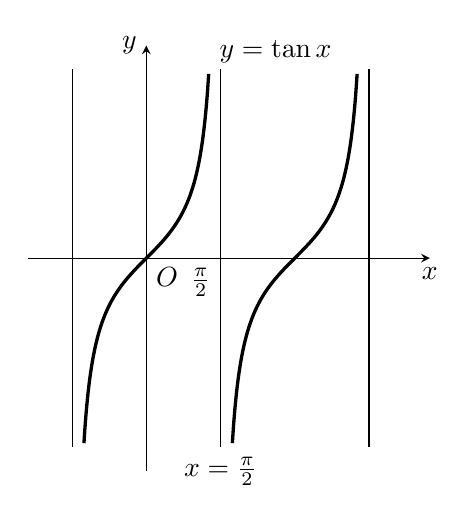
\begin{tikzpicture}[>=stealth, scale=.6]
    \draw[->](-2.5,0)--(6,0)node[below]{$x$};
    \draw[->](0,-4.5)--(0,4.5)node[left]{$y$};
\draw[domain=-pi/2+.25:pi/2-.25, very thick, smooth, samples=100]plot(\x, {tan(\x r)})node[above right]{$y=\tan x$};
\draw[domain=-pi/2+.25:pi/2-.25, very thick, smooth, samples=100]plot(\x+pi, {tan(\x r)});
\foreach \x in {-1,1,3}
{
    \draw(\x*pi/2,-4)--(\x*pi/2,4);
}
\node at (pi/2,0)[below left]{$\frac{\pi}{2}$};
\node at (pi/2,-4)[below]{$x=\frac{\pi}{2}$};
\node [below right]{$O$};
\end{tikzpicture}  
\captionof{figure}{}
\end{minipage}


点$x=0$是函数$y=\begin{cases}\frac{|x|}{x},& x\neq0 \\0,& x=0\end{cases}$的间断点(如图11.10).

\noindent
\begin{minipage}{.45\textwidth}
\centering
\begin{tikzpicture}[>=stealth]
    \draw[->](-3,0)--(3,0)node[below]{$x$};
    \draw[->](0,-2)--(0,2)node[left]{$y$};
\draw[very thick](0,1)node[left]{1}--(2.5,1)node[above]{$y=\frac{|x|}{x}$};
\draw[very thick](0,-1)node[right]{$-1$}--(-2.5,-1);
\node[below left]{$O$};
\foreach \x in {-1,1}
{
    \draw[fill=white](0,\x) circle(1.5pt);
}

\end{tikzpicture}  
\captionof{figure}{}
\end{minipage}\hfill
\begin{minipage}{.45\textwidth}
\centering
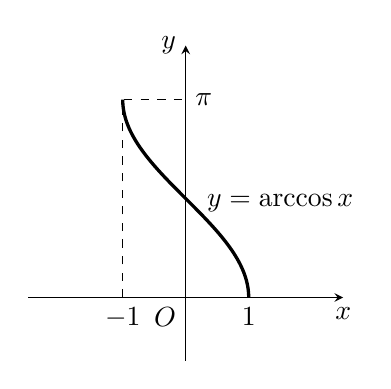
\begin{tikzpicture}[>=stealth, scale=.8]
    \draw[->](-2.5,0)--(2.5,0)node[below]{$x$};
    \draw[->](0,-1)--(0,4)node[left]{$y$};
\draw[domain=0:pi, samples=100, very thick, smooth]plot({cos(\x r)}, \x);
\foreach \x in {-1,1}
{
    \node at (\x,0)[below]{$\x$};
}
\draw[dashed](-1,0)--(-1,pi)--(0,pi)node[right]{$\pi$};
\node[below left]{$O$};
\node at (1.5,1.5){$y=\arccos x$};
\end{tikzpicture}  
\captionof{figure}{}
\end{minipage}

如果函数$y=f(x)$在点$x=x_0$处及其左侧附近有定义,并且$\Lim{x}{x^-_0}f(x)=f(x_0)$,那么称函数$f(x)$在点$x=x_0$处左连
续;如果函数$y=f(x)$在点$x=x_0$处及其右侧附近有定义,并且$\Lim{x}{x^+_0}f(x)=f(x_0)$,那么称函数$f(x)$在点$x=x_0$处右连续.
例如:函数$y=\arccos x$在点$x=1$处左连续;在点$x=-1$处右连续(如图11.11).

我们引入函数$f(x)$在一点连续和不连续的概念,反映了一个函数在一种条件下可能平稳地变化,而在另一种条件下就可能不是这样. $f(x)$在点$x=x_0$处连续的特点是当自变量$x$的值变化很小时,函数$f(x)$相应的值也变化很小;而$f(x)$在间断点$x=x_0$处的特点是自变量$x$的值变化很小时,函数$f(x)$相应的值发生很大的变化.

函数$y=f(x)$的间断点,通常是分段函数定义域区间的分界点,或者是使$f(x)$的解析式中分母的值为零的点等.

\begin{example}
已知函数$f(x)=\begin{cases}
    \sqrt{x-1},& x\geqslant1\\
    \sqrt{1-x^{2}},& 0\leqslant x<1\\
    -\sqrt{1-x^{2}},& -1\leqslant x<0
\end{cases}$
研究函数在下列各点处的连续性. 
\begin{multicols}{3}
\begin{enumerate}[(1)]
    \item $x=1$;
    \item $x=0$;
    \item $x=-1$.
\end{enumerate}
\end{multicols}
\end{example}

\begin{solution}
    函数 $y=f(x)$的图象(如图11.12)

\noindent
\begin{minipage}{.58\textwidth}
\begin{enumerate}[(1)]
    \item $\because\quad $函 数 $f( x)$在 点 $x= 1$ 处 及 附 近 有 定 义 , 并 且 $\Lim{x}{1}f( x) = f(1)=0$

$\therefore\quad $函数 $f(x)$在点 $x=1$ 处连续.
\item $\because\quad \Lim{x}{0^+}f(x)=1$, $\Lim{x}{0^-} f(x)=-1$

$\therefore\quad $函数$f(x)$在点$x=0$处不连续. 即点$x=0$是$f(x)$的间断点.
\item $\because\quad $函数$f(x)$在点$x=-1$处及右侧附近有定义,且$\Lim{x}{-1^+} f(x)=f(-1)=0$.

$\therefore\quad $函数在点$x=-1$处右连续.
\end{enumerate}    
\end{minipage}\hfill
\begin{minipage}{.4\textwidth}
\centering
\begin{tikzpicture}[>=stealth]
    \draw[->](-1.5,0)--(3.5,0)node[below]{$x$};
    \draw[->](0,-2)--(0,2.5)node[left]{$y$};
\draw[very thick](-1,0)node[above]{$-1$} arc (-180:-90:1)node[right]{$-1$};
\node[below left]{$O$};
\draw[very thick](0,1)node[left]{$1$} arc (90:0:1)node[below]{$1$};
\draw[domain=1:3.25, smooth, very thick]plot(\x, {sqrt(\x-1)});
\draw[fill=white](0,-1) circle(1.5pt);
\draw[fill](0,1) circle(1.5pt);
\end{tikzpicture}
\captionof{figure}{}
\end{minipage}    
\end{solution}

下面利用函数在某一点处连续的概念来定义连续函数.

如果函数$f(x)$在区间$(a,b)$内每一点处都连续,则称函数$f(x)$在区间$(a,b)$内连续,或者称函数$f(x)$是区间$(a,b)$内的连续函数.

如果函数$f(x)$在开区间$(a,b)$内连续,且在左端点$x=a$处右连续,在右端点$x=b$处左连续,则称函数$f(x)$在闭区间$[a,b]$上连续.

\begin{example}
    指出下列函数是否为给定区间上的连续函数?
\begin{enumerate}[(1)]
    \item $f(x)=2x^2-3x+5,\qquad x\in (-\infty,+\infty)$
    \item $f(x)=\log_2 x,\qquad x\in (0,+\infty)$
    \item $f(x)=\sqrt{2-x^2},\qquad x\in \left[-\sqrt{2},\sqrt{2}\right]$
\end{enumerate}
\end{example}

\begin{solution}
    (1)、(2)、(3)中的函数都是给定区间上的连续函数.
\end{solution}

\begin{ex}
\begin{enumerate}
    \item 已知函数$y=f(x)$的图象如下图所示,请将符合下述性质的函数图象的代号A、B、C、D分别填在指定位置。
\begin{enumerate}[(1)]
    \item $f(x)$在点$x=a$处有定义,但极限不存在的是\blank ;
    \item $f(x)$在点$x=a$处没有定义,且极限也不存在的是\blank ;
       \item $f(x)$在点$x=a$处有定义、有极限,但是$\Lim{x}{a}f(x)\ne f(a)$的是\blank ;
    \item $f(x)$在点$x=a$处没有定义,但极限存在的是\blank . 
\end{enumerate}
\begin{center}
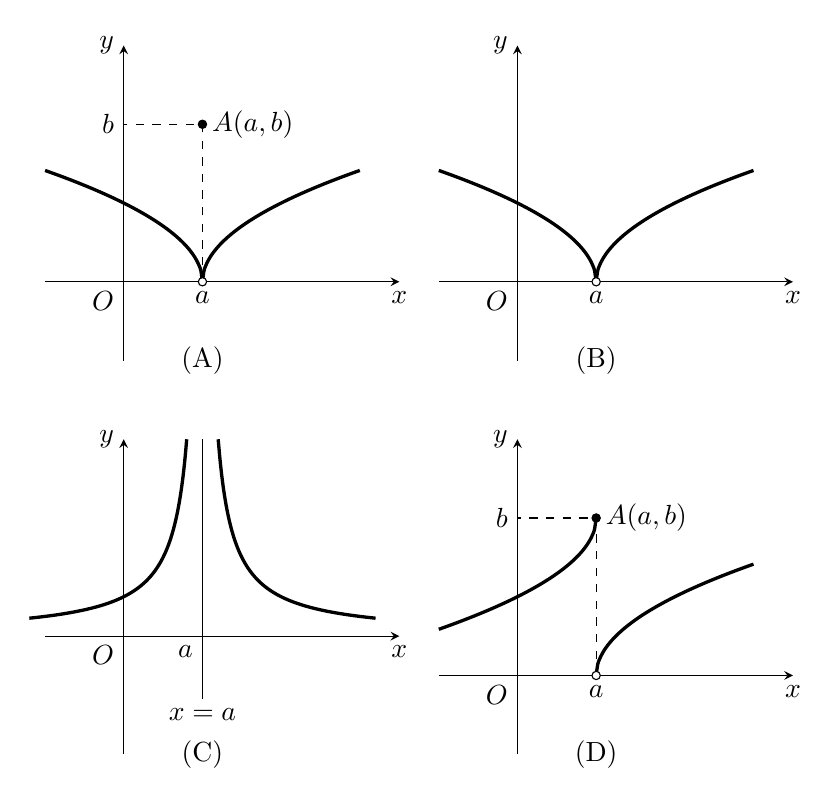
\begin{tikzpicture}[>=stealth]
\begin{scope}
\draw[->](-1,0)--(3.5,0)node[below]{$x$};
\draw[->](0,-1)--(0,3)node[left]{$y$};
\draw[domain=0:2, smooth,very thick, samples=100]plot(\x+1, {sqrt(\x)});
\draw[domain=0:2, smooth,very thick, samples=100]plot(-\x+1, {sqrt(\x)});
\node [below left]{$O$};
\node at (1,0)[below]{$a$};
\draw[dashed](1,0)--(1,2)node[right]{$A(a,b)$}--(0,2)node[left]{$b$};
\draw[fill](1,2)circle (1.5pt);
\draw[fill=white](1,0)circle (1.5pt);
\node at (1,-1){(A)};
\end{scope}
\begin{scope}[xshift=5cm]
    \draw[->](-1,0)--(3.5,0)node[below]{$x$};
\draw[->](0,-1)--(0,3)node[left]{$y$};
\draw[domain=0:2, smooth,very thick, samples=100]plot(\x+1, {sqrt(\x)});
\draw[domain=0:2, smooth,very thick, samples=100]plot(-\x+1, {sqrt(\x)});
\node [below left]{$O$};
\node at (1,0)[below]{$a$};
\draw[fill=white](1,0)circle (1.5pt);
\node at (1,-1){(B)};

\end{scope}
\begin{scope}[yshift=-4.5cm]
    \draw[->](-1,0)--(3.5,0)node[below]{$x$};
    \draw[->](0,-1.5)--(0,2.5)node[left]{$y$};
\draw(1,-.8)node[below]{$x=a$}--(1,2.5);
\node at (1,-1.5){(C)};
\node [below left]{$O$};
\node at (1,0)[below left]{$a$};
\draw[domain=0.2:2.2, smooth,very thick, samples=100]plot(\x+1, {.5/\x});
\draw[domain=0.2:2.2, smooth,very thick, samples=100]plot(-\x+1, {.5/\x});


\end{scope}
\begin{scope}[yshift=-5cm, xshift=5cm]
    \draw[->](-1,0)--(3.5,0)node[below]{$x$};
\draw[->](0,-1)--(0,3)node[left]{$y$};
\draw[domain=0:2, smooth,very thick, samples=100]plot(\x+1, {sqrt(\x)});
\draw[domain=0:2, smooth,very thick, samples=100]plot(-\x+1, -{sqrt(\x)}+2);
\node [below left]{$O$};
\node at (1,0)[below]{$a$};
\draw[dashed](1,0)--(1,2)node[right]{$A(a,b)$}--(0,2)node[left]{$b$};
\draw[fill](1,2)circle (1.5pt);
\draw[fill=white](1,0)circle (1.5pt);
\node at (1,-1){(D)};
\end{scope}
\end{tikzpicture}
\captionof*{figure}{第1题}
\end{center}

\item 指出下列函数在给定点处是否连续.
\begin{enumerate}[(1)]
    \item $f(x)=\sqrt{x+1}$,点$x=-1$;
    \item $f(x)=x^2-3x+2$,点$x=2$;
    \item $f(x)=\log_{\tfrac{1}{2}}x$,点$x=1$;
    \item $f(x)=\frac{x-1}{\sqrt{x}-1}$,点$x=1$;
    \item $f(x)=ax^2+bx+c\; (a\ne 0)$,点$x=-\frac{b}{2a}$.
\end{enumerate}
\item 指出下列函数的间断点.
\begin{multicols}{2}
\begin{enumerate}[(1)]
    \item $f(x)=\frac{1}{x^2-3x+2}$
    \item $f(x)=\frac{2x+1}{x-3}$
    \item $f(x)=\frac{x^2-4}{x-2}$
    \item $f(x)=\begin{cases}
        2^x, & x\ge 0\\ 0,& x<0
    \end{cases}$
\end{enumerate}
\end{multicols}
\end{enumerate}
\end{ex}


\section{连续函数的性质}
在客观世界中存在许多连续变化的数量,连续函数反映了这类事物中变量之间的关系.

连续函数有以下性质:

\begin{thm}{性质1}
    若函数$y=f(x)$在区间$(a,b)$内连续,$x_0\in (a,b)$,则$\Lim{x}{x_0}f(x)=f(x_0)$
\end{thm}

利用函数$f(x)$在点$x=x_0$处连续的定义,求$\Lim{x}{x_0}f(x)$的问题可转化为求$f(x_0)$的值.

\begin{thm}{性质2}
    如果函数$f(x)$、$g(x)$在某一点$x=x_0$处连续,那么函数$f(x)\pm g(x)$, $f(x)\cdot g(x)$以及$\frac{f(x)}{g(x)}\; (g(x)\ne 0)$在点$x=x_0$处都连续(此性质利用函数极限的四则运算法则不难证明).
\end{thm}

这个性质告诉我们,连续函数的和、差、积、商仍是连续函数.

\begin{thm}{性质3}
    已知函数$y=f[g(x)]$是由函数$y=f(u)$、$u=g(x)$复合而成的函数,若函数$u=g(x)$在点$x=x_0$处连续、$u_0=g(x_0)$,且函数$y=f(u)$在点$u=u_0$处也连续,则函数$y=f[g(x)]$在点$x=x_0$处也连续. 即
\[\Lim{x}{x_0} f[g(x)]=f\left[\Lim{x}{x_0} g(x)\right]=f[g(x_0)]  \]
\end{thm}

这个性质给出了求复合函数极限的一种方法.

\begin{example}
    求下列各函数的极限.
\begin{multicols}{2}
\begin{enumerate}[(1)]
    \item $\Lim{x}{3}(2x^2+5x-1)$
    \item $\Lim{x}{2}\sqrt{x^2-2}$
\end{enumerate}
\end{multicols}
\end{example}

\begin{solution}
\begin{enumerate}[(1)]
    \item $\Lim{x}{3}(2x^2+5x-1)=2\x 3^2+5\x 3-1=32$
    \item $\Lim{x}{2}\sqrt{x^2-2}=\sqrt{\Lim{x}{2}(x^2-2)}=\sqrt{2^2-2}=\sqrt{2}$
\end{enumerate}
\end{solution}    

\begin{thm}{性质4}
    若函数$y=f(x)$在区间$(a,b)$内连续,则函数$y=f(x)$在区间$(a,b)$内的图象是一条连续曲线.
\end{thm}

\begin{example}
    作下列各函数的图象
\begin{enumerate}[(1)]
    \item $y= -(|x|-1)^2+2 ,\qquad x\in \left[-\frac{3}{2},\frac{3}{2}\right]$
    \item $y= 2^{x-1}-1 ,\qquad x\in (-1,2)$
    \item $y=x^2-4x+3  ,\qquad x\in \left[0,4\right]$
\end{enumerate}
\end{example}

\begin{solution}
所作函数的图象分别为图11.13中的(1)、(2)、(3)图.
\begin{figure}[htp]
    \centering
\begin{tikzpicture}[>=stealth, scale=.9]
\begin{scope}
    \draw[->](-2,0)--(2,0)node[below]{$x$};
    \draw[->](0,-1)node[below]{(1)}--(0,3)node[left]{$y$};
\node [below left]{$O$};
\draw[domain=0:1.5, smooth, very thick]plot(\x, -\x*\x+2*\x+1);
\draw[domain=0:1.5, smooth, very thick]plot(-\x, -\x*\x+2*\x+1);
\draw[dashed](1,0)node[below]{1}--(1,2)node[above]{$A(1,2)$};
\draw[dashed](-1,0)node[below]{$-1$}--(-1,2)node[above]{$B(-1,2)$};
\draw[dashed](1.5,0)node[below]{$\tfrac{3}{2}$}--(1.5,1.75);
\draw[dashed](-1.5,0)node[below]{$-\tfrac{3}{2}$}--(-1.5,1.75);
\node at (0,1)[left]{1};
\foreach \x in {1,2}
{
    \draw(0,\x)--(.1,\x);
}

\end{scope}
\begin{scope}[xshift=4cm]
    \draw[->](-1.5,0)--(2.5,0)node[below]{$x$};
    \draw[->](0,-1)--(0,2)node[left]{$y$};
\node [below left]{$O$};
\foreach \x in {1,2}
{
    \node at (\x,0)[below]{\x};
}
\draw[dashed](2,0)node[below]{2}--(2,1)node[above]{$A(2,1)$}--(0,1)node[left]{1};
\draw[dashed](-1,0)node[above]{$-1$}--(-1,-.75)node[below]{$B(-1,-\tfrac{3}{4})$};
\draw[domain=-1:2, smooth, very thick]plot(\x, {2^(\x-1)-1});
\draw[fill=white](2,1)circle (1.5pt);
\draw[fill=white](-1,-.75)circle (1.5pt);
\node at (.5,-1)[below]{(2)};

\end{scope}
\begin{scope}[xshift=8cm, scale=.6]
    \draw[->](-1.5,0)--(5,0)node[below]{$x$};
    \draw[->](0,-2)--(0,4.5)node[left]{$y$};
\node [below left]{$O$};
\draw[domain=0:4, smooth, very thick]plot(\x, {(\x-2)^2-1})node[above]{$A(4,3)$};
\foreach \x in {1,3,4}
{
    \node at (\x,0)[below]{\x};
}
\foreach \x in {-1,1,2}
{
    \draw(0,\x)--(.1,\x);
}
\node at (2,-2)[below]{(3)};


\draw[dashed](2,0)--(2,-1)node[below]{$O'(2,-1)$};
\draw[dashed](4,0)--(4,3);
\node at (0,3)  [left]{$3$};
\end{scope}
\end{tikzpicture}
    \caption{}
\end{figure}





    
\end{solution}

观察例11.11中3个函数的图象,我们发现,第(1)、(3)个函数在给定的闭区间上都存在着最大值和最小值,而第(2)个函
数没有最大值和最小值.

\begin{thm}{性质5}
    如果$f(x)$是\textbf{闭区间}$[a,b]$上的连续函数,那么在区间$[a,b]$上\textbf{至少存在}两个点$x=x_1$、$x=x_2$,使得$f(x_1)\ge f(x)$且$f(x_2)\le f(x)$.(最大值和最小值存在定理)
\end{thm}

这个性质告诉我们,定义在闭区间上的连续函数一定有最大值和最小值,但并未解决如何求这个函数$f(x)$的最大值点和最小值点的问题.

观察例11.11中3个函数的图象我们还可以发现,当自变量$x$的值在给定区间内变化时,若使对应的函数值$f(x)$由负变正(或由正变负),则在它们中间一定存在一个点$x_0$,使得$f(x_0)=0$.

\begin{thm}{性质6}
    如果函数$f(x)$在闭区间$[a,b]$上连续,且$f(a)\cdot f(b)<0$,则在\textbf{闭区间}$[a,b]$上\textbf{至少存在}一点$C$,使得$f(c)=0$.(中间值定理).
\end{thm}

像上一个性质一样,这个中间值定理也只告诉我们使$f(c)=0$的存在性,但又启发我们可反复利用这个“中间值定理”,用逼近的方法求方程$f(x)=0$根的近似值.







\begin{example}
    利用“中间值定理”解方程$x^3-3=0$(精确到
0.001)
\end{example}

\begin{solution}
设函数 $f(x)=x^3-3$, 它的零点为 $x=\alpha$, 则 $\alpha$ 是方程
$x^3-3=0$的解

$\because\quad f( 1) = - 2< 0,\quad  f( 2) = 5> 0$

$\therefore\quad 1< \alpha < 2$ 

又$\because\quad f( 1. 4) = - 0.256< 0,\quad  f(1.5) = 0.375> 0$ 

$\therefore\quad 1.4< \alpha < 1.5$ 

又$\because\quad f( 1. 44) \approx - 0. 014< 0,\quad  f( 1. 45) \approx 0. 048> 0$

$\therefore\quad 1.44<\alpha<1.45$

又$\because\quad f( 1. 442) \approx - 0. 00156< 0$, 
$f(1.443)\approx0.0045>0$

$\therefore\quad 1. 442< \alpha < 1. 443$

又$\because\quad f( 1. 4422) \approx - 0. 0003< 0$, 
$f(1.4423)\approx0.0003>0$

$\therefore\quad 1. 4422< \alpha < 1. 4423$

$\therefore\quad $ 方程 $x^3-3=0$ 的根 $x\approx1.442$(精确到 0.001)
\end{solution}

\begin{ex}
\begin{enumerate}
    \item 求下列函数的极限:
\begin{multicols}{2}
\begin{enumerate}[(1)]
    \item $\Lim{x}{7}\sqrt[3]{x+1}$
    \item $\Lim{x}{1}\log_2(x^2+3)$
    \item $\Lim{x}{3}2^{x-1}$
    \item $\Lim{x}{0}\frac{(1+x)^2-1}{x}$
\end{enumerate}
\end{multicols}
\item 判断下列命题是否为真命题:
\begin{enumerate}[(1)]
\item 若函数$f(x)$在点$x=x_0$处连续,则当$x\to x_0$时,$f(x)-f(x_0)\to 0$.
\item 若函数$f(x)$在点$x=x_0$处连续,函数$g(x)$虽有定义但在点$x=x_0$处不连续,则$f(x)+g(x)$在点$x=x_0$处不连续.
\item 若函数$f(x)$、$g(x)$在点$x=x_0$处都有定义且都不连续,则$f(x)+g(x)$在点$x=x_0$处不连续.
\item 若函数$f(x)$在区间$(a,b)$内连续,则函数$|f(x)|$在区间$(a,b)$内也连续.
\item 若函数$f(x)$在区间$(a,b)$内是连续函数,则$f(x)$在区间$(a,b)$内有最大值和最小值.
\item 对于函数$f(x)$,若在其定义域内有两点$x=a$和$x=b$,使得$f(a)\cdot f(b)<0$,则在区间$[a,b]$上必存在一点$C$,使得$f(C)=0$.
\end{enumerate}

\item 求证:方程$7x^3+19x^2+x-2=0$有一根在区间$(0,1)$内.
\end{enumerate}
\end{ex}

\section{初等函数及其极限}

我们学过的基本函数可以分为以下5类:
\begin{enumerate}
\item 幂函数$y=x^{a}$($a$是实数);
\item 指数函数$y=a^x$($a>0$且$a\ne 1$);
\item 对数函数$y=\log_a x$($a>0$且$a\ne 1$);
\item 三角函数$y=\sin x$, $y=\cos x$, $y=\tan x$, $y=\cot x$, $y=\sec x$和$y=\csc x$.
\item 反三角函数$y=\arcsin x$, $y=\arccos x$, $y=\arctan x$, $y={\rm arccot\, }x$等.
\end{enumerate}

上述5种函数统称基本初等函数.

由基本初等函数经过\textbf{有限次}四则运算和\textbf{有限次}复合所得到的函数,统称初等函数.

\begin{example}
    试用3个基本初等函数$\lg x$、$e^x$、$x^2$构造5个初等函数.
\end{example}

\begin{solution}
    例如:
\[\begin{split}
    f_1(x)&=\lg(e^x)^2\\
    f_2(x)&=e^{\lg x}-3x^2\\
    f_3(x)&=(\lg x)^2-3\lg x\\
    f_4(x)&=e^{x^2}(x^2+e^x)\\
    f_5(x)&=3\lg^4 x-5\lg^3x+2\lg^2x-\lg x+\frac{2}{\lg x}
\end{split}\]
\end{solution}

由基本初等函数的连续性和连续函数的性质,可以推出:\textbf{一切初等函数在它们定义区间上都分别是连续函数}.

有了初等函数是连续函数的结论,不仅使我们对函数的性质有了进一步的了解,而且利用连续函数的性质,为我们研究问题带来一些方便. 比如求初等函数的极限,若函数$y=f[g(x)]$是初等函数,点$x=x_0$是它的定义区间内的一点,则
\[\lim_{x\to x_0}f[g(x)]=f\left[\lim_{x\to x_0}g(x)\right]=f[g(x_0)]\]
例如:
\[\lim_{x\to\tfrac{\pi}{2}}(\ln \sin x)=\ln\left(\lim_{x\to\tfrac{\pi}{2}}\sin x\right)=\ln\sin\frac{\pi}{2}=\ln 1=0\]
\[\LIM{x}\frac{\sqrt{2+x}-\sqrt{2}}{x}=\LIM{x}\frac{\sqrt{\frac{2}{x^2}+\frac{1}{x}}-\sqrt{\frac{2}{x^2}}}{1}=0\]
\[\begin{split}
    \Lim{x}{0}\frac{\sqrt{2+x}-\sqrt{2}}{x}&= \Lim{x}{0}\frac{(2+x)-2}{x\left(\sqrt{2+x}+\sqrt{2}\right)}\\
    &= \Lim{x}{0} \frac{1}{\sqrt{2+x}+\sqrt{2}}=\frac{1}{\sqrt{ \Lim{x}{0}(2+x)}+\sqrt{2}}\\
    &=\frac{1}{\sqrt{2}+\sqrt{2}}=\frac{\sqrt{2}}{4}
\end{split}\]

求函数的极限时,有时还可用下面这个“两面夹”定理.

\begin{thm}{定理}
 如果函数$f(x)$、$g(x)$、$h(x)$在点$x=x_0$附近满足:
\begin{enumerate}[(1)]
\item $g(x)\le f(x)\le h(x)$;
\item $\Lim{x}{x_0}g(x)=\Lim{x}{x_0}h(x)=A$($A$为常数).
\end{enumerate}
那么,$\Lim{x}{x_0}f(x)=A$.   
\end{thm}

这就是说,如果直接求一个函数$f(x)$的极限有困难,那么可以用放缩的方法,使$f(x)$夹在另外两个简单函数之间,只要这两个函数有相同的极限,$f(x)$的极限也就随之得到.


\begin{example}
求$\LIM{x}\frac{\cos x}{x}$.
\end{example}

\begin{solution}
$\because\quad $当$x\to \infty$时, $-\frac{1}{x}\le \frac{\cos x }{x}\le \frac{1}{x}$

而$\LIM{x}\left(-\frac{1}{x}\right)=0$,$\LIM{x}\frac{1}{x}=0$

$\therefore\quad \LIM{x}\frac{\cos x}{x}=0.$
\end{solution}

\section*{习题二}
\begin{center}
    \bfseries A
\end{center}

\begin{enumerate}
    \item (口答)下列初等函数分别是由哪几个基本初等函数复合而成的?
\begin{multicols}{2}
  \begin{enumerate}[(1)]
 \item $y=\sqrt[5]{\ln^2\cos x}$
\item $y=\log_2 \frac{1}{x}$   
\item $y=\left(\frac{1}{3}\right)^{x^2}$
\item $y=\arctan(\sin x^3)$
\end{enumerate}  
\end{multicols}

    \item (口答)下列初等函数是由哪些基本初等函数经过哪些四则运算得出的?
\begin{multicols}{2}
\begin{enumerate}[(1)]
    \item $y=x^4-4x^3+6x^2-4x+1$
    \item $y=\frac{2\ln x+x^2}{x-\sqrt{x}}$
    \item $y=(\arcsin x+\arccos x)^2$
    \item $y=\frac{e^x-e^{-x}}{2}$
\end{enumerate}
\end{multicols}
\item 求下列函数的连续区间:
\begin{multicols}{2}
\begin{enumerate}[(1)]
    \item $y=\frac{x}{1-\sin x}$
    \item $y=\arccos\frac{1}{x}$
    \item $y=\sqrt{2x^2+5x-3}$
    \item $y=\lg(1-e^{x+2})$
\end{enumerate}
\end{multicols}

\item 求下列函数的极限:
\begin{multicols}{2}
\begin{enumerate}[(1)]
    \item $\Lim{x}{\tfrac{\pi}{6}}(1-\sin x)^2$
    \item $\Lim{x}{2}\log_3 (2x^2+1)$
    \item $\Lim{x}{0}\frac{9^x-1}{3^x-1}$
    \item $\Lim{x}{0}\frac{(1+x)^3-1}{x}$
\end{enumerate}
\end{multicols}


\end{enumerate}

\begin{center}
    \bfseries B
\end{center}
\begin{enumerate}\setcounter{enumi}{4}
    \item 求下列各极限:
\begin{multicols}{2}
\begin{enumerate}[(1)]
    \item $\Lim{x}{ 0}\frac{\sin^2 x}{1-\cos x}$
    \item $\Lim{x}{\tfrac{\pi}{2}}\frac{2\cos x}{\sin 2x}$
    \item $\Lim{x}{16 }\frac{\sqrt[4]{x}-2}{\sqrt{x}-4}$
    \item $\Lim{x}{2 }\frac{\sqrt{2x-2}-\sqrt{x}}{x^2-4}$
    \item $\Lim{x}{ x_0}\frac{x^3-x^3_0}{x-x_0}$
    \item $\Lim{x}{x_0 }\frac{\sqrt{x}-\sqrt{x_0}}{x-x_0}$
    \item $\Lim{x}{0 }\frac{\sqrt[3]{1+x}-1}{x}$
    \item $\Lim{x}{0 }\frac{(2+x)^{-2}-2^{-2}}{x}$
\end{enumerate}
\end{multicols}

\item \begin{enumerate}[(1)]
    \item 求证$f(x)=x^4-12x^3+46x^2-60x+9$在区间$[1,5]$上有最大值和最小值.
    \item 求证方程$x^3-6x-3=0$在区间$[2,3]$内至少有一实根.
\end{enumerate}

\item \begin{enumerate}[(1)]
 \item 求证:当$x\to 0$时,$\frac{3^x}{5}<\frac{2^x+3^x}{5}<2\left(\frac{3^x}{5}\right)$
    \item 计算$\Lim{x}{0}\left(\frac{2^x+3^x}{3}\right)^{\tfrac{1}{x}}$   
\end{enumerate}
\end{enumerate}

\section{两个重要极限}
本节介绍在微积分中经常用到的两个重要的极限.

\subsection{$\Lim{x}{0}\frac{\sin x}{x}=1$}


\noindent
\begin{minipage}{.55\textwidth}
    \CTEXindent
虽然当$x\to 0$时,$\sin x\to 0$且$x\to 0$,但不能用消去分子、分母的公因式的方法来求极限. 因此想到能否利用“两面夹”定理来求这个极限.

如图11.14,在单位圆中,以$Ox$为始边的圆心角$\angle XOA=x$(其中$0<|x|<\frac{\pi}{2}$)的终边交单位圆于$A$. 作$AC\bot Ox$轴于$C$,作切线$AD$交$Ox$轴于$D$,则
\[\overline{CA}=\sin x,\quad \wideparen{TA}=x,\quad \overline{DA}=\tan x\]
\end{minipage}\hfill
\begin{minipage}{.45\textwidth}
  \centering
\begin{tikzpicture}[>=stealth, scale=1.5]
\draw[->](-1.5,0)--(1.75,0)node[below]{$x$};
\draw[->](0,-1.5)--(0,1.5)node[left]{$y$};
\draw(0,0)node[below left]{$O$} circle (1);
\tkzDefPoint(35:1){A}
\tkzDefPoints{1.22/0/D, 0.82/0/C, 1/0/T, 0/0/O}
\tkzDefPoint(-35:1){A'}
\draw[dashed, thick](0,0)--(A')--(D);
\draw[thick](0,0)--(A)--(A');
\draw[thick](A)--(D);
\tkzLabelPoints[below](A',D)
\tkzLabelPoints[above](A)
\tkzLabelPoints[above right](T)
\tkzLabelPoints[below left](C)
\tkzMarkRightAngle[size=.1](A,C,O)
\end{tikzpicture}  
\captionof{figure}{}
\end{minipage}

延长$AC$交单位圆于$A'$点,连结$OA'$, $A'D$

$\because\quad |AA'|<\wideparen{ATA'}<|AD|+|A'D|$

$\therefore\quad 2\sin x<2x<2\tan x\quad (x>0)$
或$2\sin x>2x>2\tan x\quad (x<0)$.

$\because\quad 0<|x|<\frac{\pi}{2}$

$\therefore\quad 2\sin x\ne 0$,
不等式变为
\[
    1<\frac{x}{\sin x}<\frac{1}{\cos x}\qquad  1>\frac{\sin x}{x}>\cos x
\]

$\because\quad \Lim{x}{0}1=1,\quad \Lim{x}{0}\cos x=1$

$\therefore\quad \Lim{x}{0}\frac{\sin x}{x}=1$

\begin{rmk}
由于在微积分中三角函数的自变量都是实数,因此它对应于以\textbf{弧度}为单位的角或弧.
\end{rmk}

\begin{example}
求下列极限
\begin{multicols}{2}
\begin{enumerate}[(1)]
    \item $\Lim{x}{\infty}\left(x\sin\frac{1}{x}\right)$
    \item $\Lim{x}{0}\frac{\sin 5x}{3x}$
    \item $\Lim{x}{0}\frac{\tan x}{x}$
    \item $\Lim{x}{0}\frac{1-\cos 2x}{x^2}$
\end{enumerate}
\end{multicols}
\end{example}

\begin{solution}
\begin{enumerate}[(1)]
    \item $\Lim{x}{\infty}\left(x\sin\frac{1}{x}\right)=\Lim{\tfrac{1}{x}}{0}\frac{\sin\frac{1}{x}}{\frac{1}{x}}=1$
    \item $\Lim{x}{0}\frac{\sin 5x}{3x}=\Lim{5x}{0}\frac{5\sin 5x}{3(5x)}=\frac{5}{3}\Lim{5x}{0}\frac{\sin 5x}{5x}=\frac{5}{3}$
    \item $\Lim{x}{0}\frac{\tan x}{x}=\Lim{x}{0}\frac{\sin x}{x\cos x}=\Lim{x}{0}\frac{\sin x}{x}\cdot \Lim{x}{0}\frac{1}{\cos x}=1\x 1=1$
    \item $\Lim{x}{0}\frac{1-\cos 2x}{x^2}=\Lim{x}{0}\frac{2\sin^2 x}{x^2}=2\Lim{x}{0}\left(\frac{\sin x}{x}\right)^2=2\left(\Lim{x}{0}\frac{\sin x}{x}\right)^2=2\x 1^2=2$
\end{enumerate}
\end{solution}

\subsection{$\Lim{x}{\infty}\left(1+\frac{1}{x}\right)^x=e$}
我们从下表先观察当$x\to +\infty$时函数$\left(1+\frac{1}{x}\right)^x$的变化趋势.

\begin{center}
\begin{tabular}{ccc}
\hline
    $x$ & $\left(1+\frac{1}{x}\right)^x$ & 近似值\\
\hline
1   &  $\left(1+\frac{1}{1}\right)^1$ & 2\\
10   &  $\left(1+\frac{1}{10}\right)^{10}$ &2.59374\\
100   &  $\left(1+\frac{1}{100}\right)^{100}$ &2.70481\\
1000   &  $\left(1+\frac{1}{1000}\right)^{1000}$ &2.71692\\
10000   &  $\left(1+\frac{1}{10000}\right)^{10000}$ &2.71815\\
100000   &  $\left(1+\frac{1}{100000}\right)^{100000}$ &2.71827\\
……&……& $2.71828\cdots$\\
\hline
\end{tabular}
\end{center}


可以证明,当$x\to +\infty$时,$\left(1+\frac{1}{x}\right)^x$趋近于无理数$2.718281828459045\cdots$,记作$e$.即
\[\Lim{x}{+\infty}\left(1+\frac{1}{x}\right)^x=e\]
无理数$e$和$\pi$一样,都是数学中应用最广泛的两个超越常数,很多自然规律是以$e$为底的指数函数. 当无理数$e$作为对数的底数时,这个对数又称为自然对数,正数$x$的自然对数用$\ln x$表示.

还可以证明,$\Lim{x}{\infty}\left(1+\frac{1}{x}\right)^x=e$

\begin{example}
求下列极限: 
\begin{multicols}{2}
\begin{enumerate}[(1)]
    \item $\Lim{x}{0}(1+x)^{\tfrac{1}{x}}$
    \item $\Lim{x}{\infty}\left(1+\frac{1}{x}\right)^{-x}$
    \item $\Lim{x}{\infty}\left(1-\frac{2}{x}\right)^x$
    \item $\Lim{x}{\infty}\left(1+\frac{1}{x-2}\right)^x$
\end{enumerate}
\end{multicols}
\end{example}

\begin{solution}
\begin{enumerate}[(1)]
    \item $\Lim{x}{0}(1+x)^{\tfrac{1}{x}}=\Lim{\tfrac{1}{x}}{\infty}\left(1+\frac{1}{\frac{1}{x}}\right)^{\tfrac{1}{x}}=e$
    \item $\Lim{x}{\infty}\left(1+\frac{1}{x}\right)^{-x}=\frac{1}{\Lim{\tfrac{1}{x}}{\infty}\left(1+\frac{1}{x}\right)^x}=\frac{1}{e}$
    \item \[\begin{split}
        \Lim{x}{\infty}\left(1-\frac{2}{x}\right)^x&=\Lim{x}{\infty}\left(1+\frac{1}{-\frac{x}{2}}\right)^{-\tfrac{x}{2}\cdot (-2)}\\
        &=\left[\Lim{-\tfrac{x}{2}}{\infty}\left(1+\frac{1}{-\frac{x}{2}}\right)^{-\tfrac{x}{2}}\right]^{-2}=e^{-2}
    \end{split}\]
    \item \[\begin{split}
        \Lim{x}{\infty}\left(1+\frac{1}{x-2}\right)^x&=\Lim{x}{\infty}\left(1+\frac{1}{x-2}\right)^{(x-2)+2}\\
        &=\Lim{(x-2)}{\infty}\left(1+\frac{1}{x-2}\right)^{x-2}\cdot \Lim{x}{\infty}\left(1+\frac{1}{x-2}\right)^2\\
        &=e\x 1=e
    \end{split}\]
\end{enumerate}
\end{solution}

\begin{example}
求下列极限:
\begin{multicols}{2}
\begin{enumerate}[(1)]
    \item $\Lim{x}{0}\frac{\sin\left(\frac{\pi}{3}+x\right)-\sin\frac{\pi}{3}}{x} $
    \item $\Lim{x}{0}\frac{\ln(2+x)-\ln 2}{x} $
\end{enumerate}
\end{multicols}
\end{example}

\begin{solution}
\begin{enumerate}[(1)]
    \item \[\begin{split}
\text{原式}= \lim_{x\to 0}\frac{2\cos\left(\frac{\pi}{3}+\frac{\pi}{2}\right)\sin\frac{x}{2}}{x}&= \lim_{x\to 0}\left[\frac{\sin\frac{x}{2}}{\frac{x}{2}}\cdot \cos\left(\frac{\pi}{3}+\frac{x}{2}\right)\right]\\
&= \lim_{\tfrac{x}{2}\to 0}\frac{\sin\frac{x}{2}}{\frac{x}{2}}\cdot  \lim_{\tfrac{x}{2}\to 0}\cos\left(\frac{\pi}{3}+\frac{x}{2}\right)\\
&=1\x \cos\frac{\pi}{3}=\frac{1}{2}      
    \end{split}\]
\item \[\begin{split}
\lim_{x\to 0}\frac{\ln(2+x)-\ln 2}{x}&=\lim_{x\to 0}\left[\frac{1}{x}\ln\left(1+\frac{x}{2}\right)\right]=\lim_{x\to 0}\left[\ln\left(1+\frac{1}{\frac{2}{x}}\right)^{\tfrac{1}{x}}\right]\\
&=\lim_{\tfrac{2}{x}\to \infty}\left[\ln\left(1+\frac{1}{\frac{2}{x}}\right)^{\tfrac{2}{x}}\right]^{\tfrac{1}{2}}=\lim_{\tfrac{2}{x}\to \infty}\left[\frac{1}{2}\ln\left(1+\frac{1}{\frac{2}{x}}\right)^{\tfrac{2}{x}}\right]\\
&=\frac{1}{2}\ln\left[\lim_{\tfrac{2}{x}\to \infty}\left(1+\frac{1}{\frac{2}{x}}\right)^{\tfrac{2}{x}}\right]=\frac{1}{2}\ln e=\frac{1}{2}
\end{split}\]
\end{enumerate}
\end{solution}


\begin{example}
计算$\Lim{x}{0}\frac{e^x-1}{x}$
\end{example}

\begin{solution}
    令$t=e^x\; (t>0)$,则$x=\ln t$
\[\begin{split}
    \Lim{x}{0}\frac{e^x-1}{x}&=\lim_{t\to 1}\frac{t-1}{\ln t}=\lim_{t\to 1}\frac{1}{\frac{1}{t-1}\ln\left(1+\frac{1}{\frac{1}{t-1}}\right)}=\lim_{t\to 1}\frac{1}{\ln\left(1+\frac{1}{\frac{1}{t-1}}\right)^{\tfrac{1}{t-1}}}\\
    &=\frac{1}{\Lim{\tfrac{1}{t-1}}{\infty} \left[\ln \left(1+\frac{1}{\frac{1}{t-1}}\right)^{\tfrac{1}{t-1}} \right] }=\frac{1}{\ln \left[\Lim{\tfrac{1}{t-1}}{\infty} \left(1+\frac{1}{\frac{1}{t-1}}\right)^{\tfrac{1}{t-1}} \right] }\\
&=\frac{1}{\ln e}=1
\end{split}\]
\end{solution}

\begin{ex}
\begin{enumerate}
    \item 求下列各极限:
\begin{multicols}{2}
\begin{enumerate}[(1)]
    \item $\Lim{x}{0} \frac{\sin 3x}{\sin 4x}$
    \item $\Lim{x}{0} \frac{\tan 2x}{3x}$
    \item $\Lim{x}{0} \frac{1-\cos 2x}{x\sin x}$
    \item $\Lim{x}{0} \frac{\sin5x-\sin3x}{\sin x}$
    \item $\Lim{x}{\infty} x\sin\frac{5}{x}$
    \item $\Lim{x}{\tfrac{\pi}{2}} \frac{\cos x}{\frac{\pi}{2}-x}$
\end{enumerate}
\end{multicols}

\item 求下列各极限:
\begin{multicols}{2}
    \begin{enumerate}[(1)]
        \item $\Lim{x}{\infty}\left(1+\frac{m}{x}\right)^{mx} $
        \item $\Lim{x}{0}\left(1+\tan x\right)^{\cot x} $
        \item $\Lim{x}{\infty} \left(1+\frac{1}{x}\right)^{x+2}$
        \item $\Lim{x}{0} \left(1-\frac{1}{x}\right)^{2x}$
    \end{enumerate}
\end{multicols}

\item 求下列各极限:
\begin{multicols}{2}
    \begin{enumerate}[(1)]
        \item $\Lim{x}{0} \frac{\cos\left(\frac{\pi}{3}+x\right)-\cos\frac{\pi}{3}}{x}$
        \item $\Lim{x}{0} \frac{\sin(\alpha+x)-\sin\alpha}{x}$
        \item $\Lim{x}{0} \frac{\ln(3+x)-\ln 3}{x}$
    \end{enumerate}
\end{multicols}
\end{enumerate}    
\end{ex}

\section{本章小结}

\subsection{主要内容}
本章的主要内容是函数极限的概念及其运算法则;函数连续的概念及连续函数的性质;初等函数的连续性以及二个重要的极限. 即
\[\lim_{x\to 0}\frac{\sin x}{x}=1,\qquad \lim_{x\to \infty}\left(1+\frac{1}{x}\right)^x=e\]


\subsection{函数的极限}
极限是描述函数在无限过程中的变化趋势的重要概念. 对于一般函数$f(x)$,涉及的极限过程有两类,即$x\to +\infty$、$x\to-\infty$、$x\to \infty$和$x\to x_0$、$x\to x_0^+$、$x\to x_0^-$. 在上述的任一过程中,若$f(x)$的极限存在,即$f(x)\to A$($A$为常数),则$f(x)=A+a(x)$(其中$a(x)\to 0$). 反之,在上述的任一过程中,若$f(x)
=A+a(x)$(其中$a(x)\to 0$,$A$为常数),则$f(x)\to A$,即$f(x)$的极限存在.

函数$f(x)$在点$x=x_0$处连续是利用极限$\Lim{x}{x_0}f(x)$来定义的,但是二者有区别:

$f(x)$在点$x=x_0$处的极限可用来研究$f(x)$在点$x=x_0$处附近的变化趋势,与$f(x)$在点$x=x_0$¡处是否有定义或取什么值无关.

$f(x)$在点$x=x_0$处连续不仅要求$\Lim{x}{x_0}f(x)$存在,而且要求$\Lim{x}{x_0}f(x)=f(x_0)$. 换句话说,$f(x)$在点$x=x_0$处连续就是$x\to x_0$时,$f(x)-f(x_0)\to 0$.

\subsection{求函数的极限}
求函数的极限是本章的重点内容,除了根据极限的定义求函数的极限外,目前我们已掌握的方法主要有:

\begin{enumerate}
    \item  利用函数的连续性求极限.

    若函数$f(x)$在点$x=x_0$处连续,则$\Lim{x}{x_0}f(x)=f(x_0)$.

如果复合函数$y=f[g(x)]$在点$x=x_0$处连续,则$\Lim{x}{x_0}f[g(x)]=f\left[\Lim{x}{x_0}g(x)\right]=f[g(x_0)]$.
\item 利用“两面夹定理”求极限.

若$x\to x_0$时,$g(x)\le f(x)\le h(x)$,且$\Lim{x}{x_0}g(x)=\Lim{x}{x_0}h(x)=A$($A$为常数),则
$\Lim{x}{x_0}f(x)=A$.

\begin{rmk}
    若极限过程改为$x\to \infty$等,两面夹定理仍成立.
\end{rmk}

\item 利用“两个重要极限”求极限.
\item 利用极限的四则运算法则求极限.

函数的和、差、积、商的极限利用极限的运算法则可转化为函数极限的和、差、积、商.而转化的前提是各函数的极限存在且使变形后的解折式有意义.对于那些不能直接利用极限运算法则的式子(又称为未定式),需注意掌握常用的变形方法,使得变形后的式子能利用法则、定理求极限.
\item 利用换元法求极限

换元法是数学解题中常用的方法,通过变量代换可使问题的本质看得更清楚.
\end{enumerate}

\subsection{连续函数}
一切初等函数在它们的定义区间上是连续函数.

函数的连续性是函数的又一个重要性质,应重视对连续函数性质的研究.


\section*{复习题十一}
\begin{center}
    \bfseries A
\end{center}

\begin{enumerate}
    \item (口答)指出下列各命题是真命题,还是假命题.
\begin{enumerate}[(1)]
\item 如果函数$f(x)$在点$x=x_0$处连续,那么$\Lim{x}{x_0}f(x)$存在;
\item 如果$\Lim{x}{x_0}f(x)$存在,那么函数$f(x)$在点$x=x_0$处连续;
\item 若函数$f(x)$在点$x=x_0$处连续,则当$x\to x_0$时,$f(x)-f(a)\to 0$;
\item 若$\Lim{x}{x_0}f(x)=A$,则当$x\to x_0$时,$f(x)-A\to 0$;
\item 若函数$f(x)$的定义域是实数集$\R$,则$f(x)$是连续函数;
\item 函数$f(x)=|x-1|$在点$x=1$处连续,但$\Lim{x}{1}\frac{|x-1|}{x-1}$不存在;
\item 函数$f(x)=(x+1)^2$在点$x=1$处连续,且$\Lim{x}{1}\frac{(x+1)^2-2^2}{x-1}$存在;
\item 存在这样的函数$f(x)$,它在定义域内的每一点处都不连续.
\end{enumerate}

\item 求下列函数的极限:
\begin{multicols}{2}
\begin{enumerate}[(1)]
    \item $\Lim{x}{1}\sqrt{10-x} $
    \item $\Lim{x}{3}\frac{x}{\sqrt{1+x}} $
    \item $\Lim{x}{3}\frac{x^2-9}{x^2-3x} $
    \item $\Lim{x}{\infty}\frac{x^2-9}{x^2-3x} $
    \item $\Lim{x}{\infty}\frac{-1+\sqrt{1+x}}{x} $
    \item $\Lim{x}{0}\frac{-1+\sqrt{1+x}}{x} $
    \item $\Lim{x}{\infty}\frac{3x^2+x-2}{2x^2+5x+3} $
    \item $\Lim{x}{-1}\frac{3x^2+x-2}{2x^2+5x+3} $
    \item $\Lim{x}{3}\left(\frac{12}{x^2-9}-\frac{2}{x-3}\right) $
    \item $\Lim{x}{4}\frac{\sqrt{x-2}-\sqrt{2}}{\sqrt{2x+1}-3} $
    \item $\Lim{x}{\tfrac{3\pi}{4}} \frac{\cos 2x}{\cos x+\sin x}$
    \item $\Lim{x}{0} \frac{\sin 5x-\sin 3x}{\sin x}$
    \item $\Lim{x}{\infty}x\sin\frac{2}{x} $
    \item $\Lim{x}{0} \frac{\sqrt{x+4}-2}{\sin 5x}$
    \item $\Lim{x}{\infty}\left(\frac{x+1}{x-1}\right)^x $
\end{enumerate}
\end{multicols}
\end{enumerate}

\begin{center}
    \bfseries B
\end{center}

\begin{enumerate}\setcounter{enumi}{2}

\item 求下列函数的极限:
\begin{multicols}{2}
\begin{enumerate}[(1)]
\item $\Lim{x}{0} \frac{\sin\left(\sqrt{1+x}-1\right)}{x}$
\item $\Lim{x}{0} \frac{\tan x-\sin x}{\sin^3 x}$
\item $\Lim{x}{1} \frac{\sin \pi x}{x-1}$
\item $\Lim{x}{1} \frac{\ln x}{x-1}$
\end{enumerate}
\end{multicols}


\item 求下列函数的极限:
\begin{multicols}{2}
\begin{enumerate}[(1)]
    \item $\Lim{x}{0} \frac{(a+x)^4-a^4}{x}$
    \item $\Lim{x}{0} \frac{\sqrt{a+x}-\sqrt{a}}{x}$
    \item $\Lim{x}{0} \frac{\sin 2(\alpha+x)-\sin 2\alpha}{x}$
    \item $\Lim{x}{0} \frac{\ln(a+x)-\ln a}{x}$
\end{enumerate}
\end{multicols}

\item 求证:方程$x\cdot 3^x-2=0$在区间$(0,1)$内存在一实数根.
\item 已知$\Lim{x}{2} \frac{x^2+ax+b}{x-2}=3$. 求$a$、$b$的值.
\item 已知$f(x)=\begin{cases}
    x^2+1, & x<0\\
    x-1,& 0\le x\le 2\\
    (x-1)^2, & x>2
\end{cases}$

求此函数的连续区间,并作出其图象.








\end{enumerate}
